% BEGIN LICENSE BLOCK
% Version: CMPL 1.1
%
% The contents of this file are subject to the Cisco-style Mozilla Public
% License Version 1.1 (the "License"); you may not use this file except
% in compliance with the License.  You may obtain a copy of the License
% at www.eclipse-clp.org/license.
% 
% Software distributed under the License is distributed on an "AS IS"
% basis, WITHOUT WARRANTY OF ANY KIND, either express or implied.  See
% the License for the specific language governing rights and limitations
% under the License. 
% 
% The Original Code is  The ECLiPSe Constraint Logic Programming System. 
% The Initial Developer of the Original Code is  Cisco Systems, Inc. 
% Portions created by the Initial Developer are
% Copyright (C) 2006 Cisco Systems, Inc.  All Rights Reserved.
% 
% Contributor(s): 
% 
% END LICENSE BLOCK

%\documentclass[11pt,a4paper]{book}
%\usepackage{alltt}
%\usepackage{graphics}
%%\usepackage{html}
%\topmargin 0cm
%\oddsidemargin 0cm
%\evensidemargin 0cm
%\textwidth 16cm
%\textheight 22.5cm
%
%% Allow underscores as normal characters (but lose subscripts...)
%% [moved into include file because of latex2html problem]
%%\catcode`_=\active
%
%\def\eclipse{ECL$^i$PS$^e$}
%
%% Don't use a style file for sepiachip because latex2html ignores it
%
%\makeindex
%
%\begin{document}
%
%\title{{\huge Search in ECLiPSe}}
%\author{Joachim Schimpf \and Kish Shen \and Mark Wallace}
%
%\maketitle
%%\abstract{
%%This tutorial is an overwiew of different search methods to Prolog,
%%and how to implement them in ECLiPSe.
%%}
%
%\tableofcontents

%\chapter{Search Methods}
%----------------------------------------------------------------------
\section{Introduction}
%----------------------------------------------------------------------
In this tutorial we will take a closer look at the principles and
alternative methods of searching for solutions in the presence of
constraints. Let us first recall what we are talking about.
We assume we have the standard pattern of a constraint program:
\begin{quote}\begin{alltt}
solve(Data) :-
        model(Data, Variables),
        search(Variables),
        print_solution(Variables).
\end{alltt}\end{quote}
The model part contains the logical {\em model} of our problem. It defines
the variables and the constraints.
Every variable has a {\em domain} of values that it can take
(in this context, we only consider domains with a finite number of values).

Once the model is set up, we go into the search phase.
Search is necessary since generally the implementation of the constraints
is not complete, i.e.\ not strong enough to logically infer directly
the solution to the problem. Also, there may be multiple solutions
which have to be located by search, e.g.\ in order to find the best one.
In the following, we will use the following terminology:
\begin{itemize}
\item If a variable is given a value (from its domain, of course),
        we call this an {\em assignment}. If every problem variable is given
        a value, we call this a {\em total assignment}.
\item A total assignment is a {\em solution} if it satisfies all the
        constraints.
\item The {\em search space} is the set of all possible total assignments.
        The search space is usually very large because it grows exponentially
        with the problem size:
        \begin{displaymath}
        SearchSpaceSize = {DomainSize}^{NumberOfVariables}
        \end{displaymath}
\end{itemize}


% - - - - - - - - - - - - - - - - - - - - - - - - - - - - - - - - - - -
\subsection{Overview of Search Methods}
% - - - - - - - - - - - - - - - - - - - - - - - - - - - - - - - - - - -

\begin{figure}
\begin{center}

\includegraphics{search3.eps}
\end{center}
\caption{A search space of size 16}
\label{figsearchspace}
\end{figure}
Figure \ref{figsearchspace} shows a search space with N (here 16)
possible total assignments, some of which are solutions.
Search methods now differ in the way in which these assignments
are visited.
We can classify search methods according to different criteria:
\begin{description}
\item[Complete vs incomplete exploration] complete search means that the search space
    is investigated in such a way that all solutions are guaranteed to be found.
    This is necessary when the optimal solution is needed (one has to prove
    that no better solution exists). Incomplete search may be sufficient when
    just some solution or a relatively good solution is needed.
\item[Constructive vs move-based] this indicates whether the method advances
    by incrementally constructing assignments (thereby reasoning about partial
    assignments which represent subsets of the search space) or by moving
    between total assignments (usually by modifying previously explored
    assignments).
\item[Randomness] some methods have a random element while others follow
    fixed rules.
\end{description}
Here is table of a selection of search methods together with their properties:

\begin{center}
\begin{tabular}{|l|lll|}
\hline
Method&                 exploration&    assignments&    random\\
\hline
Full tree search&       complete&       constructive&   no\\
Credit search&          incomplete&     constructive&   no\\
Bounded backtrack&      incomplete&     constructive&   no\\
Limited discrepancy&    complete&       constructive&   no\\
Hill climbing&          incomplete&     move-based&     possibly\\
Simulated annealing&    incomplete&     move-based&     yes\\
Tabu search&            incomplete&     move-based&     possibly\\
Weak commitment&        complete&       hybrid&         no\\
\hline
\end{tabular}
\end{center}

The constructive search methods usually organise the search space by
partitioning it systematically.  This can be done naturally with a
search tree (Figure \ref{figsearchtree}).  The nodes in this tree
represent choices which partition the remaining search space into two
or more (usually mutually exclusive) disjoint sub-spaces.  Using such
a tree structure, the search space can be traversed systematically and
completely (with as little as O(N) memory requirements).

\begin{figure}
\begin{center}
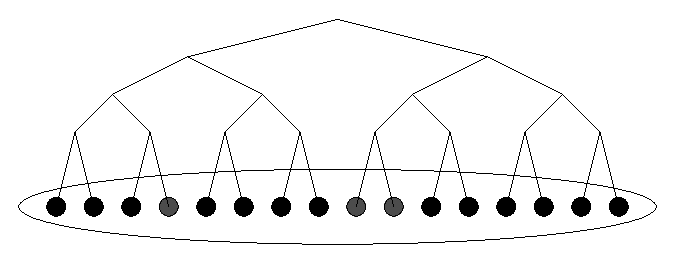
\includegraphics{search4.eps}
\end{center}
\caption{Search space structured using a search tree}
\label{figsearchtree}
\end{figure}
Figure \ref{figtreesearch} shows a sample tree search, namely a depth-first
incomplete traversal.
As opposed to that, figure \ref{figmovesearch} shows an example of an
incomplete move-based search which does not follow a fixed search space
structure. Of course, it will have to take other precautions to avoid
looping and ensure termination.
\begin{figure}
\begin{center}
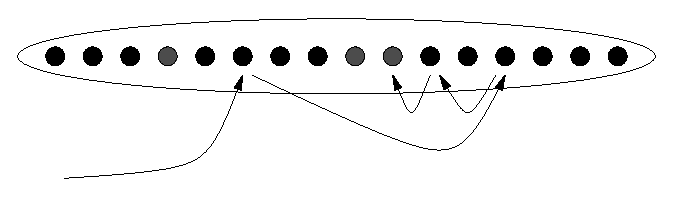
\includegraphics{search5.eps}
\end{center}
\caption{A move-based search}
\label{figmovesearch}
\end{figure}

\begin{figure}
\begin{center}
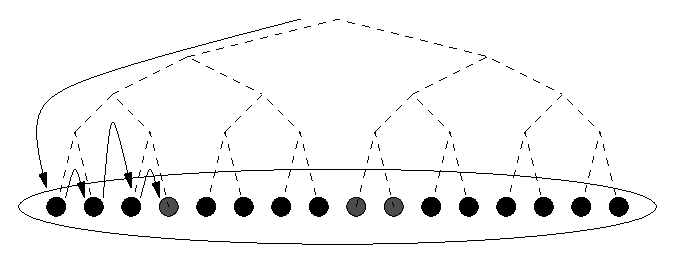
\includegraphics{search6.eps}
\end{center}
\caption{A tree search (depth-first)}
\label{figtreesearch}
\end{figure}

A few further observations:
Move-based methods are usually incomplete. This is not surprising given
typical sizes of search spaces.
A complete exploration of a huge search space
is only possible if large sub-spaces can be excluded a priory, and this
is only possible with constructive methods which allow to reason about
whole classes of similar assignments.
Moreover, a complete search method must remember which parts of the
search space have already been visited.
This can only be implemented with
acceptable memory requirements if there is a simple structuring of the
space that allows compact encoding of sub-spaces.


% - - - - - - - - - - - - - - - - - - - - - - - - - - - - - - - - - - -
\subsection{Optimisation and Search}
% - - - - - - - - - - - - - - - - - - - - - - - - - - - - - - - - - - -

Many practical problems are in fact optimisation problems, ie.\ we are
not just interested in some solution or all solutions, but in
the best solution.

Fortunately, there is a general method to find the optimal solution
based on the ability to find all solutions.
\index{branch-and-bound}
The {\em branch-and-bound} technique works are follows:
\begin{enumerate}
\item Find a first solution
\item Add a constraint requiring a better solution than the best
    one we have so far (e.g.\ require lower cost)
\item Find a solution which satisfies this new constraint.
    If one exists, we have a new best solution and we repeat step 2.
    If not, the last solution found is the proven optimum.
\end{enumerate}
The library {\bf branch\_and\_bound} provides the generic
branch-and-bound primitives bb\_min/3 and bb\_min/6.


% - - - - - - - - - - - - - - - - - - - - - - - - - - - - - - - - - - -
\subsection{Heuristics}
% - - - - - - - - - - - - - - - - - - - - - - - - - - - - - - - - - - -

Since search space sizes grow exponentially with problem size,
it is not possible to explore all assignments except for the
very smallest problems.
The only way out is {\em not} to look at the whole search space.
There are only two ways to do this:
\begin{itemize}
\item {\bf Prove} that certain areas of the space contain no solutions.
    This can be done with the help of constraints. This is often referred
    to as {\em pruning}\index{pruning}.
\item {\bf Ignore} parts of the search space that are unlikely to contain
    solutions (i.e.\ do incomplete search), or at least postpone their exploration.
    This is done by using {\em heuristics}\index{heuristics}.
    A heuristic is a particular traversal order of the search space
    which explores promising areas first.
\end{itemize}

In the following sections we will first investigate the considerable
degrees of freedom that are available for heuristics within the framework of
systematic tree search, which is the traditional search method
in the Constraint Logic Programming world.

Subsequently, we will turn our attention to move-based methods
which in {\eclipse} can be implemented using the facilities of the repair-library.


%----------------------------------------------------------------------
\section{Complete Tree Search with Heuristics}
%----------------------------------------------------------------------

There is one form of tree search which is especially economic: 
depth-first, left-to-right search by backtracking.  It allows to
traverse a search tree systematically while requiring only a stack
of maximum depth N for bookkeeping.  Most other strategies of tree
search (e.g.  breadth-first) have exponential memory requirements. 
This unique property is the reason why backtracking is a built feature
of {\eclipse}.  Note that the main disadvantage of the depth-first
strategy (the danger of going down an infinite branch) does not come
into play here because we deal with finite search trees.

Sometimes depth-first search and heuristic search are treated as antonyms.
This is only justified when the shape of the search tree is statically fixed.
Our case is different: we have the freedom of deciding on the shape of every
sub-tree before we start to traverse it depth-first. While this does not
allow to arrange for {\em any} order of visiting the leaves of the search tree,
it does provide considerable flexibility. This flexibility can be exploited
by variable and value selection strategies.

% - - - - - - - - - - - - - - - - - - - - - - - - - - - - - - - - - - -
\subsection{Search Trees}
% - - - - - - - - - - - - - - - - - - - - - - - - - - - - - - - - - - -

In general, the nodes of a search tree represent {\em choices}.
\index{choice}
These choices should be mutually exclusive and therefore partition the
\index{partition a search space}
search space into two or more disjoint sub-spaces.
In other words, the original problem is reduced to a disjunction
of simpler sub-problems.

In the case of finite-domain problems, the most common form of choice
is to choose a particular value for a problem variable
(this technique is often called
\index{labeling}
{\em labeling}).
For a boolean variable, this means setting the variable to 0 in one
branch of the search tree and to 1 in the other.
In {\eclipse}, this can be written as a disjunction
(which is implemented by backtracking):
\begin{quote}\begin{alltt}
( X1=0 ; X1=1 )
\end{alltt}\end{quote}
Other forms of choices are possible. If X2 is a variable that can take
integer values from 0 to 3 (assume it has been declared as \verb'X2::0..3'),
we can make a n-ary search tree node by writing
\begin{quote}\begin{alltt}
( X2=0 ; X2=1 ; X2=2 ; X2=3 )
\end{alltt}\end{quote}
or more compactly
\begin{quote}\begin{alltt}
indomain(X2)
\end{alltt}\end{quote}
However, choices do not necessarily involve choosing a concrete value
for a variable. It is also possible to make disjoint choices by
\index{domain splitting}
{\em domain splitting}, e.g.
\begin{quote}\begin{alltt}
( X2 #=< 1 ; X2 #>= 2 )
\end{alltt}\end{quote}
or by choosing a value in one branch and excluding it in the other:
\begin{quote}\begin{alltt}
( X2 = 0 ; X2 #>= 1 )
\end{alltt}\end{quote}
In the following examples, we will mainly use simple labeling,
which means that the search tree nodes correspond to a variable
and a node's branches correspond to the different values that the
variable can take.


% - - - - - - - - - - - - - - - - - - - - - - - - - - - - - - - - - - -
\subsection{Variable Selection}
% - - - - - - - - - - - - - - - - - - - - - - - - - - - - - - - - - - -

\begin{figure}
\begin{center}
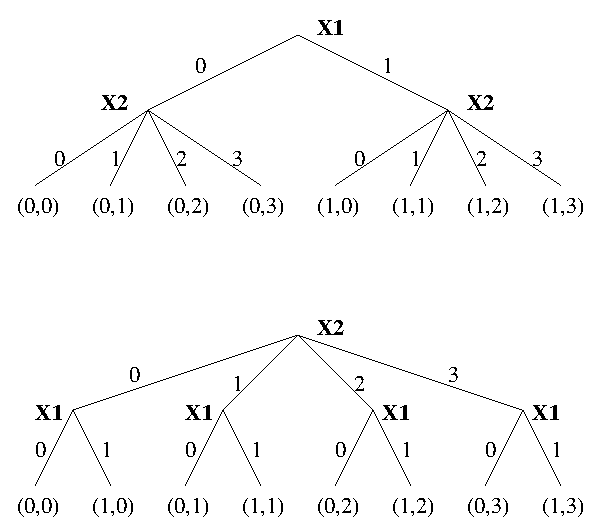
\includegraphics{search1.eps}
\end{center}
\caption{The effect of variable selection}
\label{figvarsel}
\end{figure}

Figure \ref{figvarsel} shows how variable selection reshapes a search tree.
If we decide to choose values for X1 first (at the root of the search tree)
and values for X2 second, then the search tree has one particular shape.
If we now assume a depth-first, left-to-right traversal by backtracking,
this corresponds to one particular order of visiting the leaves of the tree:
(0,0), (0,1), (0,2), (0,3), (1,0), (1,1), (1,2), (1,3).

If we decide to choose values for X2 first and X1 second, then the tree and
consequently the order of visiting the leaves is different:
(0,0), (1,0), (0,1), (1,1), (0,2), (1,2), (0,3), (1,3).

While with 2 variables there are only 2 variable selection strategies,
this number grows exponentially with the number of variables. For 5
variables there are already $2^{2^{5}-1} = 2147483648$ different variable selection
strategies to choose from.

Note that the example shows something else: If the domains of the variables
are different, then the variable selection can change the number of internal
nodes in the tree (but not the number of leaves). To keep the number of nodes
down, variables with small domains should be selected first.


% - - - - - - - - - - - - - - - - - - - - - - - - - - - - - - - - - - -
\subsection{Value Selection}
% - - - - - - - - - - - - - - - - - - - - - - - - - - - - - - - - - - -

The other way to change the search tree is value selection, i.e. reordering
the child nodes of a node by choosing the 
values from the domain of a variable in a particular order.
Figure \ref{figvalsel} shows how this can change the order of visiting the
leaves:
(1,2), (1,1), (1,0), (1,3), (0,1), (0,3), (0,0), (0,2).

\begin{figure}
\begin{center}
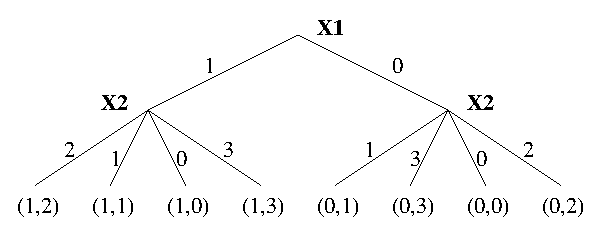
\includegraphics{search2.eps}
\end{center}
\caption{The effect of value selection}
\label{figvalsel}
\end{figure}

By combining variable and value selection, a large number of different
heuristics can be implemented.
To give an idea of the numbers involved, the following table shows the search
space sizes, the number of possible search space traversal orderings,
and the number of orderings
that can be obtained by variable and value selection (assuming domain size 2).

\enableunderscores
\begin{center}
\begin{tabular}{|l|l|l|l|}
\hline
Variables&      Search space&   Visiting orders&        Selection Strategies\\
\hline
1&              2&                      2&              2\\
2&              4&                      24&             16\\
3&              8&                      40320&          336\\
4&              16&                     $2.1*10^{13}$&  $1.8*10^7$\\
5&              32&                     $2.6*10^{35}$&  $3.5*10^{15}$\\
n&              $2^n$&          $2^n!$& 
                                $2^{{2^n}-1} \prod_{i=0}^{n-1} (n-1)^{2^i}$\\
\hline
\end{tabular}
\end{center}
\disableunderscores

% - - - - - - - - - - - - - - - - - - - - - - - - - - - - - - - - - - -
\subsection{Example}
% - - - - - - - - - - - - - - - - - - - - - - - - - - - - - - - - - - -

We use the famous N-Queens problem to illustrate how heuristics can be applied
to backtrack search through variable and value selection.
We model the problem with one variable per queen, assuming that each queen
occupies one colunm. The variables range from 1 to N and indicate the row
in which the queen is being placed. The constraints ensure that no two
queens occupy the same row or diagonal:
%!!!!!!!!!!!!!!!!!!!!!!!!!!!!!!!!!!!!!!!!!!!!!!!!!!
% CAUTION: I use the old ## syntax here because
% #\= is not treated correctly by latex2html
%!!!!!!!!!!!!!!!!!!!!!!!!!!!!!!!!!!!!!!!!!!!!!!!!!!
\begin{quote}\begin{alltt}
:- lib(fd).

queens(N, Board) :-
        length(Board, N),
        Board :: 1..N,
        ( fromto(Board, [Q1|Cols], Cols, []) do
            ( foreach(Q2, Cols), count(Dist,1,_), param(Q1) do
                noattack(Q1, Q2, Dist)
            )
        ).

    noattack(Q1,Q2,Dist) :-
        Q2 ## Q1,
        Q2 - Q1 ## Dist,
        Q1 - Q2 ## Dist.
\end{alltt}\end{quote}
We are looking for a first solution to the 16-queens problem by calling
\begin{quote}\begin{alltt}
?- queens(16, Vars),   % model
   labeling(Vars).     % search
\end{alltt}\end{quote}
We start naively, using the pre-defined labeling-predicate that comes with the
finite-domain library. It is defined as follows:
\begin{quote}\begin{alltt}
labeling(AllVars) :-
        ( foreach(Var, AllVars) do
            indomain(Var)                       % select value
        ).
\end{alltt}\end{quote}
The strategy here is simply to select the variables
from left to right as they occur in the list, and they are
assigned values starting from the lowest to the numerically highest they can
take (this is the definition of indomain/1).
A solution is found after 542 backtracks
(see section \ref{countbt} below for how to count backtracks).

A first improvement is to employ a
{\bf general-purpose variable-selection heuristic},
\index{first-fail principle}
the so called first-fail principle. It requires to label the
variables with the smallest domain first. This reduces the branching
factor at the root of the search tree and the total number of internal nodes.
The deleteff/3 predicate implements this strategy for finite domains.
Using deleteff/3, we can redefine our labeling-routine as follows:
\begin{quote}\begin{alltt}
labeling(AllVars) :-
        ( fromto(AllVars, Vars, VarsRem, []) do
            deleteff(Var, Vars, VarsRem),       % dynamic var-select
            indomain(Var)                       % select value
        ).
\end{alltt}\end{quote}
Indeed, for the 16-queens example, this leads to a dramatic improvement,
the first solution is found with only 3 backtracks now.
But caution is necessary: The 256-queens instance for example solves
nicely with the naive strategy, but our improvement leads to a
disappointment: the time increases dramatically!
This is not uncommmon with heuristics: one has to keep in mind that the
search space is not reduced, just re-shaped. Heuristics that yield good
results with some problems can be useless or counter-productive with others.
Even different instances of the same problem can exhibit widely different
characteristics.
 
Let us try to employ a {\bf problem-specific heuristic}:
Chess players know that pieces in the middle of the board are more
useful because they can attack more fields. We could therefore start
placing queens in the middle of the board to reduce the number of
unattacked fields earlier. We can achieve that simply by pre-ordering the
variables such that the middle ones are first in the list:
\begin{quote}\begin{alltt}
labeling(AllVars) :-
        middle_first(AllVars, AllVarsPreOrdered), % static var-select
        ( foreach(Var, AllVarsPreOrdered) do
            indomain(Var)                       % select value
        ).
\end{alltt}\end{quote}
The implementation of middle\_first/2 requries a bit of list manipulation
and uses primitives from the lists-library:
\begin{quote}\begin{alltt}
:- lib(lists).

middle_first(List, Ordered) :-
        halve(List, Front, Back),
        reverse(Front, RevFront),
        splice(Back, RevFront, Ordered).
\end{alltt}\end{quote}
This strategy also improves things for the 16-queens instance, the
first solution requires 17 backtracks.

We can now improve things further by {\bf combining} the two
variable-selection strategies:
When we pre-order the variables such that the middle ones are first,
the deleteff/3 predicate will prefer middle variables when several
have the same domain size:
\begin{quote}\begin{alltt}
labeling(AllVars) :-
        middle_first(AllVars, AllVarsPreOrdered), % static var-select
        ( fromto(AllVarsPreOrdered, Vars, VarsRem, []) do
            deleteff(Var, Vars, VarsRem),       % dynamic var-select
            indomain(Var)                       % select value
        ).
\end{alltt}\end{quote}
The result is positive: for the 16-queens instance,
the number of backtracks goes down to zero,
and more difficult instances become solvable!

Actually, we have not yet implemented our intuitive heuristics properly.
We start placing queens in the middle columns, but not on the middle rows.
With our model, that can only be achieved by {\bf changing the value selection},
ie.\ setting the variables to values in the middle of their domain.
We therefore invent a variant of indomain/1 called middle\_first\_indomain/1
and the resulting labeling routine then looks as follows:
\begin{quote}\begin{alltt}
labeling(AllVars) :-
        middle_first(AllVars, AllVarsPreOrdered), % static var-select
        ( fromto(AllVarsPreOrdered, Vars, VarsRem, []) do
            deleteff(Var, Vars, VarsRem),       % dynamic var-select
            middle_first_indomain(Var)          % select value
        ).
\end{alltt}\end{quote}
The implementation of middle\_first\_indomain/2
simply relies on middle\_first/2:
\begin{quote}\begin{alltt}
middle_first_indomain(X) :-
        nonvar(X).
middle_first_indomain(X) :-
        var(X),
        dom(X, List),    % the list of values in X's domain
        middle_first(List, Ordered),
        member(X, Ordered).
\end{alltt}\end{quote}
Surprisingly, this improvement again increases the backtrack count for
16-queens again to 3.
However, when looking at a number of different instances of the problem,
we can observe that the overall behaviour has improved and the
performance has become more predictable than with the
initial more naive strategies.


% - - - - - - - - - - - - - - - - - - - - - - - - - - - - - - - - - - -
\subsection{Counting Backtracks}
% - - - - - - - - - - - - - - - - - - - - - - - - - - - - - - - - - - -

%The size of the (remaining) search space can be computed easily
%in finite-domain problems. All we have to do is to multiply the
%sizes of all the (remaining) variable's domains:
%\begin{quote}\begin{alltt}
%search_space(Vars, Size) :-
%        ( foreach(V,Vars), fromto(1,S0,S1,Size) do
%            dvar_domain(V,D), S1 is S0*dom_size(D)
%        ).
%\end{alltt}\end{quote}

\label{countbt}
An interesting piece of information during program development is the
number of backtracks. It is a good measure for the quality of
both constraint propagation and search heuristics.
We can instrument our labeling routine as follows:
\begin{quote}\begin{alltt}
labeling(AllVars) :-
        init_backtracks,
        ( foreach(Var, AllVars) do
            count_backtracks,       % insert this before choice!
            indomain(Var)
        ),
        get_backtracks(B),
        printf("Solution found after %d backtracks%n", [B]).
\end{alltt}\end{quote}
The backtrack counter itself can be implemented by the code below.
It uses a non-logical counter variable (backtracks) and an additional
flag (deep\_fail) which ensures that backtracking to exhausted choices
does not increment the count.
\begin{quote}\begin{alltt}
:- local variable(backtracks), variable(deep_fail).

init_backtracks :-
        setval(backtracks,0).

get_backtracks(B) :-
        getval(backtracks,B).

count_backtracks :-
        setval(deep_fail,false).
count_backtracks :-
        getval(deep_fail,false),        % may fail
        setval(deep_fail,true),
        incval(backtracks),
        fail.
\end{alltt}\end{quote}
Note that there are other possible ways of defining the number of backtracks.
However, the one suggested here has the following useful properties:
\begin{itemize}
\item Shallow backtracking (an attempt to instantiate a variable which
    causes immediate failure due to constraint propagation) is not counted.
    If constraint propagation works well, the count is therefore zero.
\item With a perfect heuristic, the first solution is found with zero
    backtracks.
\item If there are N solutions, the best achievable value is N (one backtrack
    per solution). Higher values indicate an opportunity to improve pruning
    by constraints.
\end{itemize}


%----------------------------------------------------------------------
\section{Incomplete Tree Search}
%----------------------------------------------------------------------
%\subsection{Pruning with Extra Constraints}
%\subsection{First Solution}

% - - - - - - - - - - - - - - - - - - - - - - - - - - - - - - - - - - -
\subsection{Bounded Backtrack Search} 
% - - - - - - - - - - - - - - - - - - - - - - - - - - - - - - - - - - -

One way to limit the scope of backtrack search is to keep a
record of the number of backtracks, and curtail the search when this
limit is exceeded.

You can find an implementation of Bounded Backtrack Search ({\em BBS})
in the file {\tt lds.ecl} in the {\tt doc/examples} directory of your
{\eclipse} installation.
The predicate defining bounded backtrack search is
\verb0bounded_backtrack_search0, and it takes two arguments, a list of
variables and an integer (the limit on the number of backtracks).
An example invocation is:
\begin{quote}\begin{alltt}
?- [X,Y,Z]::1..3, X+Y+Z#=6, bounded_backtrack_search([X,Y,Z],4).
\end{alltt}\end{quote}
The answers are returned on backtracking in the following order:
\begin{itemize}
\item
X = 1
Y = 2
Z = 3
\item
X = 1
Y = 3
Z = 2  
\item
X = 2
Y = 1
Z = 3
\item
X = 2
Y = 2
Z = 2    
\end{itemize}
After which the procedure fails outputting
\verb0Backtrack limit exceeded0.

The implementation uses several
facilities of {\eclipse}, including {\em non-logical variables} and
{\em catch and throw}:
\begin{quote}\begin{alltt}
:- local variable(backtracks), variable(deep_fail).

bounded_backtrack_search(List,Limit) :-
        setval(backtracks,Limit),
        block(bbs_label(List),
              exceed_limit,
              (writeln('Backtrack limit exceeded'), fail)
             ).

bbs_label([]).
bbs_label([Var|Vars]) :-
        limit_backtracks,
        indomain(Var),
        bbs_label(Vars).
    
limit_backtracks :-
        setval(deep_fail,false).
limit_backtracks :-
        getval(deep_fail,false),        % may fail
        setval(deep_fail,true),
        decval(backtracks),
        (getval(backtracks,0) -> exit_block(exceed_limit) ; fail).
\end{alltt}\end{quote}


% - - - - - - - - - - - - - - - - - - - - - - - - - - - - - - - - - - -
\subsection{Credit Search}
% - - - - - - - - - - - - - - - - - - - - - - - - - - - - - - - - - - -

Credit search is a tree search method where the number of
nondeterministic choices is limited a priori.  This is achieved by
starting the search at the tree root with a certain integral amount of
credit.  This credit is split between the child nodes, their credit
between their child nodes, and so on.  A single unit of credit cannot
be split any further: subtrees provided with only a single credit unit
are not allowed any nondeterministics choices, only one path though these
subtrees can be explored, i.e. only one leaf in the subtree can be visited.
Subtrees for which no credit is left are pruned,
i.e.\ not visited.

The following code (a replacement for labeling/1)
implements credit search. For ease of understanding, it is
limited to boolean variables:
\begin{quote}\begin{alltt}
% Credit search (for boolean variables only)
credit_search(Credit, Xs) :-
        (
            foreach(X, Xs),
            fromto(Credit, ParentCredit, ChildCredit, _)
        do
            ( var(X) ->
                ParentCredit > 0,  % possibly cut-off search here
                ( % Choice
                    X = 0, ChildCredit is (ParentCredit+1)//2
                ;
                    X = 1, ChildCredit is ParentCredit//2
                )
            ;
                ChildCredit = ParentCredit
            )
        ).
\end{alltt}\end{quote}
Note that the leftmost alternative (here X=0)
gets slightly more credit than the rightmost one (here X=1)
by rounding the child node's credit up rather than down. 
This is especially relevant when the leftover credit is down to 1:
from then on, only the leftmost alternatives will be taken until a
leaf of the search tree is reached. The leftmost alternative should
therefore be the one favoured by the search heuristics.

What is a reasonable amount of credit to give to a search?
In an unconstrained search tree, the credit is equivalent to the
number of leaf nodes that will be reached.
The number of leaf nodes grows exponentially with the number of
labelled variables, while tractable computations should have
polynomial runtimes. A good rule of thumb could therefore be to
use as credit the number of variables squared or cubed, thus enforcing
polynomial runtime.

Note that this method in its pure form allow choices only close to the
root of the search tree and disallows choices completely below a certain
tree depth. This is too restrictive when the value selection strategy
is not good enough. A possible remedy is to combine credit search with
bounded backtrack search.


% - - - - - - - - - - - - - - - - - - - - - - - - - - - - - - - - - - -
\subsection{Timeout}
% - - - - - - - - - - - - - - - - - - - - - - - - - - - - - - - - - - -

Another form of incomplete tree search is simply to use time-outs.
The branch-and-bound primitives min\_max/6,8 and minimize/6,8 allow
to specify a maximal runtime. If a timeout occurs, the best solution
found so far is returned instead of the proven optimum.

A general timeout can be implemented as follows. When Goal has run for
more than Seconds seconds, it is aborted and TimeOutGoal is called instead.
\begin{quote}\begin{alltt}
:- set_event_handler(timeout, exit_block/1).

timeout(Goal, Seconds, TimeOutGoal) :-
        block(
            timeout_once(Goal, Seconds),
            timeout,
            call(TimeOutGoal)
        ).

    timeout_once(Goal, Seconds) :-
        event_after(timeout, Seconds),
        ( call(Goal) ->
            cancel_after_event(timeout)
        ;
            cancel_after_event(timeout),
            fail
        ).
\end{alltt}\end{quote}


%----------------------------------------------------------------------
\subsection{Limited Discrepancy Search}
%----------------------------------------------------------------------

% - - - - - - - - - - - - - - - - - - - - - - - - - - - - - - - - - - -
\subsubsection{Introduction}
% - - - - - - - - - - - - - - - - - - - - - - - - - - - - - - - - - - -

Limited discrepancy search ({\em LDS}) is a search method that assumes
the user has a good heuristic for directing the search.  A perfect
heuristic would, of course, not require any search.  However most
heuristics are occasionally misleading.  Limited Discrepancy Search
follows the heuristic on almost every decision.  The
``discrepancy'' is a measure of the degree to which it fails to follow
the heuristic.  LDS starts searching with a discrepancy of $0$ (which
means it follows the heuristic exactly).  Each time LDS fails to find
a solution with a given discrepancy, the discrepancy is increased and
search restarts.  In theory the search is complete, as eventually the
discrepancy will become large enough to admit a solution, or cover
the whole search space.  In practice, however, it is only beneficial
to apply LDS with small discrepancies.  Subsequently, if no solution
is found, other search methods should be tried.

The definitive reference to LDS is:
\begin{quote}
Limited Discrepancy Search, Harvey and Ginsberg,
pp.607-613, Proc. IJCAI'95
\end{quote}

This reference also suggests that combining LDS with Bounded Backtrack
Search ({\em BBS}) yields good behaviour.  Accordingly the {\eclipse} LDS
module also supports BBS and its combination with LDS.

% - - - - - - - - - - - - - - - - - - - - - - - - - - - - - - - - - - -
\subsubsection{Limited Discrepancy Search using a Static Heuristic}
% - - - - - - - - - - - - - - - - - - - - - - - - - - - - - - - - - - -

We start by assuming a static heuristic, which is a complete
assignment to the problem variables specified in advance of the
search.  The predicate supporting static LDS takes a list of variables
(those which are to be labelled) and a list of values (one heuristic
value for each variable, respectively).  Each variable has a finite
domain, and its heuristic value should belong to its domain (though
the LDS search can still succeed even if this is not the case).

The measure of discrepancy, in this case, is simply the number of
variables labelled differently to the heuristic.  Thus the maximum
discrepancy is just the number of variables to be
labelled.

LDS search is implemented in the file
{\tt lds.ecl} in the {\tt doc/examples} directory of your
{\eclipse} installation. You can copy this file and load it with
\begin{quote}\begin{alltt}
:- use_module(lds).
\end{alltt}\end{quote}
Static LDS search is then available via the predicate
{\bf static_lds(Var, Vals, Discrepancy)} whose arguments are
\begin{description}
\item[Vars] the list of problem variables.  Some of the
variables may already be instantiated.  The others
must have associated finite domains.
\item[Vals] the list of values according to the heuristic.  It
must be the same length as Vars, and the heuristic
must match the value, in case the variable is
already instantiated.
\item[Discrepancy] the discrepancy of the solution returned.  Typically this
is an output of the search (an integer between $0$ and the number of
variables), but it can also be used as an input.
\end{description}
The finite domain library must be loaded, and the variables must have
finite domains.  An example invocation is:
\begin{quote}\begin{alltt}
?- [X,Y,Z]::1..3, X+Y+Z#=5, static_lds([X,Y,Z],[1,2,3],D).
\end{alltt}\end{quote}
The answers are returned on backtracking in the following order:
\begin{itemize}
\item
X = 1
Y = 2
Z = 2
D = 1     
\item
X = 1
Y = 1
Z = 3
D = 1     
\item
X = 1
Y = 3
Z = 1
D = 2     
\item
X = 2
Y = 2
Z = 1
D = 2     
\item
X = 2
Y = 1
Z = 2
D = 3     
\item
X = 3
Y = 1
Z = 1
D = 3
\end{itemize}


% - - - - - - - - - - - - - - - - - - - - - - - - - - - - - - - - - - -
\subsubsection{Limited Discrepancy Search using a Dynamic Heuristic}
% - - - - - - - - - - - - - - - - - - - - - - - - - - - - - - - - - - -

Often the heuristic value is calculated on the fly, during search.  To
cope with this we use the {\eclipse} ``tentative value'' facility in
{\eclipse}'s {\em repair} library. 
The heuristic is stored with the variable as its tentative value. 

The tentative value may be changed during search.  For example if a
variable is instantiated as a consequence of constraint propagation
during search, its tentative value is automatically changed to its
actual value. 

Dynamic LDS search is available in {\eclipse} via the predicate
{\bf dynamic_lds(Vars, Discrepancy)}.
Each variable in the list of variables {\em Vars} 
must have a tentative value.

An example invocation is:
\begin{quote}\begin{alltt}
?- [X,Y,Z]::1..3, [X,Y,Z] tent_set [1,2,3], X+Y+Z#=5,
   dynamic_lds([X,Y,Z],D).
\end{alltt}\end{quote}
The answers are returned on backtracking in the following order.
Notice that the first solution has a discrepancy of $0$, because
constraint propagation instantiates the third variable to $2$,
thus changing its tentative value from $3$ to $2$.
\begin{itemize}
\item
X = 1
Y = 2
Z = 2
D = 0    
\item
X = 1
Y = 1
Z = 3
D = 1    
\item
X = 1
Y = 3
Z = 1
D = 1    
\item
X = 2
Y = 2
Z = 1
D = 1    
\item
X = 3
Y = 1
Z = 1
D = 1    
\item
X = 2
Y = 1
Z = 2
D = 2 
\end{itemize}

% - - - - - - - - - - - - - - - - - - - - - - - - - - - - - - - - - - -
\subsubsection{LDS and BBS Combined}
% - - - - - - - - - - - - - - - - - - - - - - - - - - - - - - - - - - -

The two search techniques, BBS and LDS, can be merged quite simply in
{\eclipse}, so that for each discrepancy level only a limited number of
backtracks are allowed.  

An example invocation is:
\begin{quote}\begin{alltt}
?- Vars=[X,Y,Z], Vars::1..3, Vars tent_set [1,2,3], X+Y+Z#=6,
   bbs_dynamic_lds(Vars,4,D).
\end{alltt}\end{quote}
The answers are returned on backtracking in the following order:
\begin{itemize}
\item
X = 1
Y = 2
Z = 3
D = 0   
\item
X = 1
Y = 3
Z = 2
D = 1   
\item
X = 2
Y = 2
Z = 2
D = 1   
\item
X = 3
Y = 2
Z = 1
D = 1   \\
Backtrack limit exceeded
\item
X = 2
Y = 1
Z = 3
D = 2 \\
Backtrack limit exceeded
\end{itemize}

%----------------------------------------------------------------------
\section{Local Search Methods}
%----------------------------------------------------------------------

In the following we discuss several examples of move-based (as opposed
to constructive search) methods. These methods have originally been developed
for unconstrained problems, but they work for certain classes of
constrained problems as well.

From a technical point of view, the main difference between tree search
and move-based search is that tree search is monotonic in the sense that
constraints get tightened when going down the tree, and this is undone
in reverse order when backing up the tree to a parent node. This fits
well with the idea of constraint propagation.
In a move-based search, the main characteristics is that a move produces
a small change, but it is not clear what effect this will have on the
constraints. They may become more or less satisfied.
We therefore need implementations of the constraints that monitor changes
rather than propagate instantiations. This functionality is provided by
the {\eclipse} repair library which is used in the following examples.
The repair library is decribed in more detail in the
{\eclipse} Constraint Library Manual.
 
The {\eclipse} code for all the examples in this section is available
in the file {\tt knapsack_ls.ecl} in the {\tt doc/examples} directory of your
{\eclipse} installation.

% - - - - - - - - - - - - - - - - - - - - - - - - - - - - - - - - - - -
\subsection{The Knapsack Example}
% - - - - - - - - - - - - - - - - - - - - - - - - - - - - - - - - - - -

We will demonstrate the local search methods using the well-known
knapsack problem. The problem is the following: given a container of
a given capacity and a set of items with given weights and profit
values, find out which items have to be packed into the container
such that their weights do not exceed the container's capacity and
the sum of their profits is maximal.

The model for this problem involves N boolean variables, a single
inequality constraint to ensure the capacity restriction, and an
equality to define the objective function.

The tree search program for this problem looks as follows:
\begin{quote}\begin{alltt}
:- lib(fd).
knapsack(N, Profits, Weights, Capacity, Profit) :-
        length(Vars, N),                    % N boolean variables
        Vars :: 0..1,
        Capacity #>= Weights*Vars,          % the single constraint
        Profit #= Profits*Vars,             % the objective
        min_max(labeling(Vars), -Profit).   % branch-and-bound search
\end{alltt}\end{quote}
At the end of the problem modelling code, a standard branch-and-bound tree search
(min_max) is invoked in the last line of the code.
The parameters mean
\begin{itemize}
\item {\tt N} - the number of items (integer)
\item {\tt Profits} - a list of N integers (profit per item)
\item {\tt Weights} - a list of N integers (weight per item)
\item {\tt Capacity} - the capacity of the knapsack (integer)
\item {\tt Opt} - the optimal result (output)
\end{itemize}
To be able to use local search, we load the {\bf repair} library and
change the problem setup slightly.
At the end, we invoke a local search routine instead of tree search:
\begin{quote}\begin{alltt}
:- lib(fd).
:- lib(repair).
knapsack(N, Profits, Weights, Capacity, Opt) :-
        length(Vars, N),
        Vars :: 0..1,
        Capacity #>= Weights*Vars  r_conflict cap,
        Profit tent_is Profits*Vars,
        local_search(<extra parameters>, Vars, Profit, Opt).
\end{alltt}\end{quote}
We are now using 3 features from the repair-library:
\begin{description}
\item[Constraint annotation r\_conflict:] Constraints annotated in this
        way are constantly being monitored for satifying the global
        assignment, i.e. it is checked whether they would be satisfied
        if all variables were instantiated to their tentative values.
        Constraints that are not satisfied in this way appear in the
        specified {\em conflict set}.
        In the example, the single capacity constraint has been annotated with
        {\bf r\_conflict} and it will appear in the conflict set called
        {\tt cap} when violated.
\item[Result tent\_is ArithExpression:] This is similar to the is/2 built-in
        predicate, but it works on the variable's tentative values rather
        than requiring the variables to be instantiated. The result is
        delivered as the tentative value of Result. Any change of tentative
        value inside the ArithExpression leads to an update of the Result.
        In the example, the computation of the objective function has
        been changed to use {\bf tent\_is} because we want to have the
        objective value recomputed efficiently after every move.
\item[Tentative values:] Every variable has, apart from its domain,
        a tentative value which can be changed using tent\_set/2 and
        queried using tent\_get/2. We will use these inside the local search
        routine to implement the moves.
\end{description}


% - - - - - - - - - - - - - - - - - - - - - - - - - - - - - - - - - - -
\newpage
\subsection{Search Code Schema}
% - - - - - - - - - - - - - - - - - - - - - - - - - - - - - - - - - - -

In the literature, e.g.\ in
\begin{quote}
Localizer: A Modeling Language for Local Search,
L. Michel and P. Van Hentenryck, Proceeding CP97, LNCS 1330, Springer 1997.
\end{quote}
local search methods are often characterised by
the the following nested-loop program schema:
\begin{quote}\begin{alltt}
local_search:
     set starting state
     while global_condition
         while local_condition
             select a move
             if acceptable
                 do the move
                 if new optimum
                     remember it
         endwhile
         set restart state
     endwhile
\end{alltt}\end{quote}
The actual program codes in the following sections all follow this schema,
except that some methods (random walk and the tabu search)
are even simpler and use only a single loop with a single termination
condition.


%----------------------------------------------------------------------
\newpage
\subsection{Random walk}
%----------------------------------------------------------------------

As a simple example of local search, let us look at a random walk
strategy.  The idea is to start from a random tentative assignment of
variables to 0 (item not in knapsack) or 1 (item in knapsack), then to
remove random items (changing 1 to 0) if the knapsack's capacity is
exceeded and to add random items (changing 0 to 1) if there is
capacity left.  We do a fixed number (MaxIter) of such steps and keep
track of the best solution encountered.

Each step consists of
\begin{itemize}
\item Changing the tentative value of some variable, which in turn causes
        the automatic recomputation of the conflict constraint set
        and the tentative objective value.
\item Checking whether the move lead to a solution and whether this
        solution is better than the best one so far.
\end{itemize}

Here is the {\eclipse} program. We assume that the problem has been set
up as explained above. The violation of the capacity constraint
is checked by looking at the conflict constraints. If there are no
conflict constraints, the constraints are all tentatively satisfied
and the current tentative values form a solution to the problem.
The associated profit is obtained by looking at the tentative value
of the Profit variable (which is being constantly updated by tent\_is).
\begin{quote}\begin{alltt}
random_walk(MaxIter, VarArr, Profit, Opt) :-
        init_tent_values(VarArr, random),       % starting point
        (   for(_,1,MaxIter),                   % do MaxIter steps
            fromto(0, Best, NewBest, Opt),      % track the optimum
            param(Profit,VarArr)
        do
            ( conflict_constraints(cap,[]) ->   % it's a solution!
                Profit tent_get CurrentProfit,  % what is its profit?
                (
                    CurrentProfit > Best        % new optimum?
                ->
                    printf("Found solution with profit %w%n", [CurrentProfit]),
                    NewBest=CurrentProfit       % yes, remember it
                ;
                    NewBest=Best                % no, ignore
                ),
                change_random(VarArr, 0, 1)     % add another item
            ;
                NewBest=Best,
                change_random(VarArr, 1, 0)     % remove an item
            )
        ).
\end{alltt}\end{quote}
The auxiliary predicate {\tt init_tent_values} sets the tentative values
of all variables in the array randomly to 0 or 1:
The {\tt change_random} predicate changes a randomly selected variable with
a tentative value of 0 to 1, or vice versa.
Note that we are using an array, rather than a list of variables, to
provide more convenient random access.
The complete code and the auxiliary predicate definitions can be found
in the file {\tt knapsack_ls.ecl} in the {\tt doc/examples} directory of your
{\eclipse} installation.


%----------------------------------------------------------------------
\subsection{Hill Climbing}
%----------------------------------------------------------------------

The following hill-climbing implementation is an instance of the nested
loop program schema introduced above.  The idea is to start from
a configuration which is certainly a solution (the empty knapsack)
and do random uphill moves for at most MaxIter times. Then we restart
and try again:
\begin{quote}\begin{alltt}
hill_climb(MaxTries, MaxIter, VarArr, Profit, Opt) :-
        init_tent_values(VarArr, 0),            % starting solution
        (
            for(I,1,MaxTries),
            fromto(0, Opt1, Opt4, Opt),
            param(MaxIter,Profit,VarArr)
        do
            (
                for(J,1,MaxIter),
                fromto(Opt1, Opt2, Opt3, Opt4),
                param(I,VarArr,Profit)
            do
                Profit tent_get PrevProfit,
                (
                    flip_random(VarArr),        % try a move
                    Profit tent_get CurrentProfit,
                    CurrentProfit > PrevProfit, % is it uphill?
                    conflict_constraints(cap,[])  % is it a solution?
                ->
                    ( CurrentProfit > Opt2 ->   % is it new optimum?
                        printf("Found solution with profit %w%n",
                                    [CurrentProfit]),
                        Opt3=CurrentProfit      % accept and remember
                    ;
                        Opt3=Opt2               % accept
                    )
                ;
                    Opt3=Opt2                   % reject (move undone)
                )
            ),
            init_tent_values(VarArr, 0)         % restart
        ).
\end{alltt}\end{quote}
The move operator is implemented as follows. It chooses a random variable X
from the array of variables and changes its tentative value from 0 to 1
or from 1 to 0 respectively:
\begin{quote}\begin{alltt}
flip_random(VarArr) :-
        functor(VarArr, _, N),
        X is VarArr[random mod N + 1],
        X tent_get Old,
        New is 1-Old,
        X tent_set New.
\end{alltt}\end{quote}
Some further points are worth noticing:
\begin{itemize}
\item The move operation and the acceptance test
are within the condition part of the if-then-else construct.
As a consequence, if the acceptance test fails (the move either yields
no solution or does not improve the objective) the move is automatically
undone by backtracking.
\item To check whether the move is uphill, we retrieve the tentative
value of the Profit-variable before and after the move is done. 
Remember that, since the move operator changes the tentative values of
some variable, the tent\_is/2 primitive will automatically
update the Profit variable.
\item As in the random walk example, constraint satisfaction is checked
by checking whether the conflict constraint set is empty.
\end{itemize}

%----------------------------------------------------------------------
\newpage
\subsection{Simulated Annealing}
%----------------------------------------------------------------------

Simulated Annealing is a slightly more complex variant of local search.
It follows the schema in figure \ref{figmovesearch} and uses the same
move operator as the hill-climbing example.
The differences are in the termination conditions and in the
acceptance criterion for a move.
The outer loop simulates the cooling process by reducing the temperature
variable T, the inner loop does random moves until MaxIter steps have been
done without improvement of the objective.
The acceptance criterion is the classical one for simulated annealing:
Uphill moves are always accepted, downhill moves with a probability
that decreases with the temperature. The search routine must be invoked
with appropriate start and end temperatures, they should roughly correspond
to the maximum and minimum profit changes that a move can incur.
\begin{quote}\begin{alltt}
sim_anneal(Tinit, Tend, MaxIter, VarArr, Profit, Opt) :-
        starting_solution(VarArr),              % starting solution
        (   fromto(Tinit, T, Tnext, Tend),
            fromto(0, Opt1, Opt4, Opt),
            param(MaxIter,Profit,VarArr,Tend)
        do
            printf("Temperature is %d%n", [T]),
            (    fromto(MaxIter, J0, J1, 0),
                fromto(Opt1, Opt2, Opt3, Opt4),
                param(VarArr,Profit,T)
            do
                Profit tent_get PrevProfit,
                (   flip_random(VarArr),        % try a move
                    Profit tent_get CurrentProfit,
                    exp((CurrentProfit-PrevProfit)/T) > frandom,
                    conflict_constraints(cap,[])   % is it a solution?
                ->
                    ( CurrentProfit > Opt2 ->   % is it new optimum?
                        printf("Found solution with profit %w%n",
                                    [CurrentProfit]),
                        Opt3=CurrentProfit,     % accept and remember
                        J1=J0
                    ; CurrentProfit > PrevProfit ->
                        Opt3=Opt2, J1=J0        % accept
                    ;
                        Opt3=Opt2, J1 is J0-1   % accept
                    )
                ;
                    Opt3=Opt2, J1 is J0-1       % reject
                )
            ),
            Tnext is max(fix(0.8*T),Tend)
        ).
\end{alltt}\end{quote}

%----------------------------------------------------------------------
\newpage
\subsection{Tabu Search}
%----------------------------------------------------------------------
Another variant of local search is tabu search.  Here, a number of moves
(usually the recent moves) are remembered (the tabu list) to direct the
search. Moves are selected by an acceptance criterion, with a 
different (generally stronger) acceptance crtierion for moves in the tabu
list.  As in most local search methods there are many possible variants and
concrete instances of this basic idea. For example, how a move would be
added to or removed from the tabu list has to be specified, along with the
different acceptance criteria.

In the following simple example, the tabu list has a length determined by
the parameter TabuSize. The local moves consist of either adding
the item with the best relative profit into the knapsack, or removing
the worst one from the knapsack. In both cases, the move gets rememebered
in the fixed-size tabu list, and the complementary move is forbidden
for the next TabuSize moves.
\begin{quote}\begin{alltt}
tabu_search(TabuSize, MaxIter, VarArr, Profit, Opt) :-
        starting_solution(VarArr),              % starting solution
        tabu_init(TabuSize, none, Tabu0),
        (   fromto(MaxIter, I0, I1, 0),
            fromto(Tabu0, Tabu1, Tabu2, _),
            fromto(0, Opt1, Opt2, Opt),
            param(VarArr,Profit)
        do
            (   try_set_best(VarArr, MoveId),   % try uphill move
                conflict_constraints(cap,[]),   % is it a solution?
                tabu_add(MoveId, Tabu1, Tabu2)  % is it allowed?
            ->
                Profit tent_get CurrentProfit,
                ( CurrentProfit > Opt1 ->       % is it new optimum?
                    printf("Found solution with profit %w%n", [CurrentProfit]),
                    Opt2=CurrentProfit          % accept and remember
                ;
                    Opt2=Opt1                   % accept
                ),
                I1 is I0-1
            ;
                (   try_clear_worst(VarArr, MoveId),    % try downhill move
                    tabu_add(MoveId, Tabu1, Tabu2)      % is it allowed?
                ->
                    I1 is I0-1,
                    Opt2=Opt1                   % reject
                ;
                    I1=0,                       % no moves possible, stop
                    Opt2=Opt1                   % reject
                )
            )
        ).
\end{alltt}\end{quote}

In practice, the tabu search forms only a skeleton around which a complex
search algorithm is built. An example of this is applying tabu search to
the job-shop problem, as described by Nowicki and Smutnicki ({\it A Fast
Taboo Search Algorithm for the Job Shop Problem}, Management Science/Vol.\
42, No.\ 6, June 1996). 

%----------------------------------------------------------------------
\section{Hybrid Search Methods}
%----------------------------------------------------------------------

% - - - - - - - - - - - - - - - - - - - - - - - - - - - - - - - - - - -
\subsection{Weak-commitment Search}
% - - - - - - - - - - - - - - - - - - - - - - - - - - - - - - - - - - -
\subsubsection{Introduction}
% - - - - - - - - - - - - - - - - - - - - - - - - - - - - - - - - - - -

Weak-commitment Search (WCS) can be seen as one of the simplest form of
nogood learning. It was proposed by Yokoo, and the main reference is:
\begin{quote}
Makoto Yokoo, {\it Weak-commitment Search for Solving Constraint Satisfaction
Problems}, in AAAI'94, pg. 313-318.
\end{quote}
WCS starts by giving tentative
assignments to the variables of the problem. Labelling of the variables are
then performed, guided by a heuristic that considers the tentative
values. If  a dead-end is reached,
where no value can be assigned to a variable without violating some
constraint, then the current search is abandoned, and a new search restarted
from scratch with an extra `nogood' constraint. This `nogood' constraint
remembers the previously assigned
values to the already labelled variables in the just abandoned search. This
combination of values lead to a dead-end, and will not be tried again in
the new search. This is in contrast to a conventional backtracking search,
where the search would not be entirely abandoned, but will try assigning
new alternative values to one (generally the last assigned) variable. The
`weak-commitment' refers to this feature of the search technique, wherein
it is not `strongly committed' to the current branch in the search-space as
in conventional backtracking search. The aim is that the search would not
be `stuck' exhaustively exploring a particular region of a search-space
that might not lead to a solution. The search is instead guided by the
`nogood' constraints, which are added (`learned') after each step.  

The min-conflict heuristic of Minton et al. is the heuristic used to
label variables. In this heuristics, a `probe' is performed when assigning
a value to a variable, in which all the values in the remaining domain of the
variable (i.e. values which causes no constraint violations with existing
assigned variables) are considered. The value chosen is the value that
causes the minimum conflict (constraint violation) with the tentative
values of the still unlabelled variables. 

% - - - - - - - - - - - - - - - - - - - - - - - - - - - - - - - - - - -
\subsubsection{Using the WCS}
% - - - - - - - - - - - - - - - - - - - - - - - - - - - - - - - - - - -
The code for the facilities described below is available
in the file {\tt wcs.ecl} in the {\tt doc/examples} directory of your
{\eclipse} installation.
\begin{quote}\begin{alltt}
:- compile(wcs).
\end{alltt}\end{quote}
The WCS is invoked by calling the \verb'wcs/2' predicate:
\begin{quote}\begin{alltt}
wcs(+Vars, ++Initial)
\end{alltt}\end{quote}

\noindent
where \verb'Vars' is a list of variables that are to be labelled by the
search, and \verb'Initial' is a list of the initial tentative values that
are assigned to the variables. Before calling the procedure, the user must
already have set up the initial constraints so that the search can
proceed. During the search process, additional nogood constraints would be
added to direct the search.

Two example usage of the search are given: 1) a search for potentially all
the solutions to the N-Queens problem, and 2) a search for the first
solution to the 3SAT problems, when given the constraints on the variables
in the form of Prolog facts.

The 3SAT example is simpler in that it involves only nogood constraints:
the initial constraints on the variables are simply translated into nogood
constraints before \verb'wcs/2' is called. In the N-Queens example,
additional constraints on the placement of the queens have to be specified
before \verb'wcs/2' is called.  

The constraints that are specified for the WCS have to apply to both the
tentative and actual values of the variables. Tentative values are
implemented in this predicate using the repair library, and thus the
constraints have to be made known to the repair library. This is done using
the \verb'r_prop' annotation provided by the library. With this annotation, the
repair library would apply the constraint to the tentative values as well
as to the normal values. 


% - - - - - - - - - - - - - - - - - - - - - - - - - - - - - - - - - - -
\subsubsection{Implementation of WCS}
% - - - - - - - - - - - - - - - - - - - - - - - - - - - - - - - - - - -

The WCS implementation presented here is a simple and straight-forward
implementation in {\eclipse} of the basic algorithm presented by Yokoo.
The finite domains and the repair libraries were used. The finite domain
library was used to allow for the probing step, where all valid values for
a variable are tried. The repair library was used to allow for tentative
values to be associated with variables, as specified in the algorithm.

The repair library is used in the following way:

\begin{itemize}
\item Setting up the nogood constraints to apply to both the actual and
tentative values of the variables. This is done via the \verb'r_prop'
annotation.
\item Setting the tentative value of a variable, either initially, or
updating it at each restart. This is done using \verb'tent_set/2'. 
\item  Counting the number of constraint violations on the
tentative values for remaining unlabelled variables as a variable is
labelled to a particular value. This is done via
{\tt conflict_constraints/1}.
\end{itemize}

The predicate also has to implement the probing and restart steps of the
WCS which replace the usual tree search strategy. The probing
step tries out all the possible valid values for a variable, and picks the
value which leads to the least number of conflicts (constraint violations)
with the tentative values in the unlabelled variables. This is done with
\verb'minimize/2' from the finite domains library:

\begin{quote}\begin{alltt}
label(Var) :-
       minimize((
             indomain(Var),
             conflict_constraints(Constraints),
             length(Constraints, L) ), L).
\end{alltt}\end{quote}

The above tries out the available values of \verb'Var', collect the
constraints violations on the tentative variables using
\verb'conflict_constraints' from the repair library, and counts the number
of such constraints using \verb'length/2'. The value with the minimum
number of constraint violation is selected as the binding to \verb'Var' by
this procedure.

The search restart itself is quite easy to implement in {\eclipse}, as the
just described labelling procedure, \verb'label/1', does not leave behind a
choice-point. Thus, when a dead-end is reached in labelling values, a
simple failure will cause the procedure to fail back to the beginning,
i.e. before any variable is labelled. The restart is then implemented by
specifically creating a choice-point at the start of the search, in the
\verb'do_search/2' predicate:

\begin{quote}\begin{alltt}
do_search(Vars, _) :-
        try_one_step(Vars, Vars),
        % remember solution as a nogood so it would not be tried again
        remember_nogood(Vars).
do_search(Vars, N) :- 
        % hit dead-end and failed, try again from start after recording nogoods
        add_nogood(Vars),  % put in most recent nogood
        getval(nlabels, NL),
        printf("Restart %w - labelled %w%n",[N,NL]),
        N1 is N + 1,
        do_search(Vars, N1).
\end{alltt}\end{quote}

\noindent
\verb'try_one_step/2' tries out one search, with the first argument
containing the variables remaining to be labelled (initially all the
variables), and the second argument being all the variables. This would
fail if the labelling hits a dead-end and fails. In this case, the second
clause of \verb'do_search/2' will be tried, in which a new search is
started. The only difference is that a new nogood constraint will be
remembered. Note that if \verb'try_one_step' succeeds, then a solution will
have been generated. To allow for the search of more solutions, this
solution is remembered as a nogood in the first clause of
\verb'do_search/2'. 

The main difficulty with implementing restart is to remember the values of 
labelled variables so that it can be added as a nogood. The addition of the
nogood must be done {\it after\/} the failure and backtracking from the
dead-end, so that it will not be removed by the backtracking. The problem is
that the backtracking process will also remove the bindings on the labelled
variables. Thus, some means is required to remember the nogood values from
the point just before the failure, which can then be retrieved after the
failure to produce a new nogood constraint. Not only do the values
themselves have to be remembered, but which variable a particular value is
associated with has also to be remembered. This is done using the
non-logical variable feature of {\eclipse}, which allows copies of
terms to be stored across backtracking. A non-logical variable is
declared by a \verb'variable/1' declaration:

\begin{quote}\begin{alltt}
:- local variable(varbindings).
\end{alltt}\end{quote}

\noindent
which associates the name \verb'varbindings' with a non-logical value. The
value of this variable can then be set via \verb'setval/2' and accessed
via \verb'getval/2' built-ins. In order to remember
which variable is associated with which value,  all the variables being
labelled, which is organised as a list,
are copied using \verb'setval/2'\footnote{The call to copy\_term/3 is used
to strip attributes (domains etc) from any remaining variables in Vars.}:
\begin{quote}\begin{alltt}
remember_nogood(Vars) :-
        copy_term(Vars, NVars, _),
        setval(varbindings,NVars).
\end{alltt}\end{quote}

\noindent
To remember the current labellings when a dead-end is reached, so that a
new nogood constraint can be added for the restarted search,
\verb'remember_nogood/1' is called before the actual failure is allow to occur:

\begin{quote}\begin{alltt}
label_next(Cons, Left0, Vars) :-
        pick_var(Cons, Left0, Var, Left1), 
        incval(nlabels),
        ( label(Var) ->
            try_one_step(Left1, Vars)
        ;
            remember_nogood(Vars),
            fail
        ).
\end{alltt}\end{quote}

\noindent
The routine first picks an unlabelled variable to label next, and 
if it is successful, the
routine recursively tries to label the remaining unlabelled variables. If
not, \verb'label(Var)' fails, and the else case of the if-then-else is
called to remember the nogoods before failing.

As already described, a new nogood constraint is added by the
\verb'add_nogood/1' predicate, as shown below:

\begin{quote}\begin{alltt}
add_nogood(NewConfig) :-
        getval(varbindings, Partial),
        (foreach(P, Partial), foreach(V,NewConfig), 
         fromto(NoGoods,NG0, NG1, []), fromto(NGVars,NGV0,NGV1,[]) do 
            (nonvar(P) ->
                V tent_set P,
                NG0 = [P|NG1],
                NGV0 = [V|NGV1]
            ;   NG0 = NG1,   % keep old tentative value
                NGV0 = NGV1
            )
        ),
        NoGoods ~= NGVars r_prop. % no good
\end{alltt}\end{quote}

If a variable had been labelled in the previous search, the labelled value
becomes the tentative value. Otherwise, the variable retains the original
tentative value.

The nogood constraints are implemented via the built-in sound difference
operator, \verb'~=/2'. For example, 

\begin{quote}\begin{alltt}
[A,B,C] ~= [1,2,3]
\end{alltt}\end{quote}

\noindent
states that the variables \verb'A', \verb'B' and \verb'C'
cannot take on the values of \verb'1', \verb'2' and \verb'3' respectively
at the same time. The operator will fail when \verb'[A,B,C]' becomes ground
and take on the values \verb'[1,2,3]'. If any of the variables take on a
value different from what is specified, \verb'~=/2' will (eventually)
succeed. The operator thus acts passively, waiting for the variables to be
instantiated and then check if they are taking on the `nogood' values, and
does not propagate or deduce any further information. 

The algorithm described by Yokoo does not specify how the next variable is
selected for labelling. In this routine, it is done by the
\verb'pick_var/4' predicate:

\begin{quote}\begin{alltt}
pick_var(Cons, Left0, Var, Left) :-
        term_variables(Cons, Vars0),
        deleteffc(Var0, Vars0, Vars1),
        (is_validvar(Var0, Left0, Left) ->
            Var = Var0 ; pick_var1(Vars1, Left0, Var, Left)
        ).
\end{alltt}\end{quote}

\noindent
The next variable to be labelled is chosen from the set of variables whose
tentative values are causing conflict. The repair library maintains the
(repair) constraints which are causing conflict, and any variable which are
causing conflict will occur in these constraints. The set of conflicting
repair constraints is passed to \verb'pick_var/4' in the first argument:
\verb'Cons'. \verb'term_variables' is used to obtain all the variables that
occur in these constraints. The fd predicate \verb'deleteffc' is then used
to select a variable (picking the one with the smallest domain and most
constraints), and then this variable is checked to make sure that it is
valid variable to be labelled, i.e.\ that it is one of the variables to be
labelled. The reason for this check is that it is expected that the WCS
routine will be used as part of a larger program, and the program may use
the repair library itself, and thus \verb'Cons' may contain constraints
unrelated to the WCS labelling. 

% - - - - - - - - - - - - - - - - - - - - - - - - - - - - - - - - - - -
\subsubsection{Improving Implementation of Nogoods}
% - - - - - - - - - - - - - - - - - - - - - - - - - - - - - - - - - - -

As already stated, the built-in \verb'~=/2' used for nogood constraints is
passive. More powerful propagation can be added to the nogood constraint if
the constraint is defined by the user. To try this out, a somewhat more
powerful constraint was tried out. This constraint does forward checking,
in that when only one variable specified in a nogood remains unlabelled,
and the labelled variables are labelled to the values specified by the
nogood, the constraint that this last variable cannot take on its nogood
value can be propagated. This increase the efficiency of the search in many
cases, although at the price of a slightly more complex implementation
of the nogood constraint. 

The nogood constraint is implemented as shown:
\begin{quote}\begin{alltt}
nogood([X|Xs], [V|Vs]) :-
        ( X==V ->   nogood(Xs, Vs)
        ; var(X) -> nogood(Xs, Vs, X, V)
        ;           true
        ).

    nogood([], [], X1, V1) :- X1 ## V1.
    nogood([X|Xs], [V|Vs], X1, V1) :-
        ( X==V ->   nogood(Xs, Vs, X1, V1)
        ; var(X) -> suspend(nogood([X1,X|Xs], [V1,V|Vs]), 3, X-X1->inst)
        ;           true
        ).
\end{alltt}\end{quote}
\noindent
The nogood-constraint is set up by
\begin{quote}\begin{alltt}
nogood(NGVars, NoGoods) r_prop.
\end{alltt}\end{quote}
The implementation checks whether NGVars matches NoGoods and causes
failure if this is the case. If a non-matching variable-value pair is
encountered, the constraint disappears. If a variable is encountered,
nogood/4 continues checking, and if the variable turns out to be the only
one, the corresponding values gets removed from its domain.
If a second variable is encountered, the constraint re-suspends until
at least one of them gets instantiated.

Obviously, this is still a relatively naive implementation of the
nogood-technique. As the number of nogoods grows, implementing them
via indivudual constraints will become more and more infeasible, and
optimisation techniques like merging and indexing of the nogoods
will be needed.

\end{document}
